\chapter{Планирование траекторий} \label{ch:5}

\section{Введение} \label{sect5_1}
Существует несколько различных ситуаций, в которых требуется планировать траекторию:
\begin{itemize}
	\item Траектория между несколькими точками без избегания препятствий
	\item Траектория между двумя точками без избегания препятствий
	\item Траектория между двумя точками избегающая препятствия
\end{itemize}

Первый случай - результат работы геометрического планировщика, построившего путь с учетом препятствий.
Второй случай возникает в ситуациях, когда геометрический планировщик построил путь свободный от препятствий или же известно, что они отсутствуют.
Третий случай является результатом отсутствия геометрического планировщика или быстро изменяющейся динамической среды, в которой находится много перемещающихся препятствий(к примеры многолюдное помещение и тп.п). Этот случай довольно редок на практике, поскольку удешевление микропроцессорной техники и вычислительных ресурсов привело к тому, что появилась возможность в режиме реального времени строить пути свободные от препятствий в условиях динамической среды. Поэтому этот случай рассмотрен не будет. 
Кроме того не рассмотрен случай генерирования траекторий по нескольким точкам с избеганием препятствий, потому что в этом случае путь разбивается на пары точек и используются те же самые методы, что и в траекториях между двумя точками.

\section{Планирование траекторий между несколькими точками без обхода препятствий} \label{sect5_2}
После построения планировщиком пути, необходимо построить траекторию, то есть определить динамические параметры, такие как скорость и ускорение на всем пути. Во-первых нужно получить непрерывный путь, для решения этой задачи можно использовать сплайны. Степень сплайна выбирается исходя из требований к плавности траекторий. В данной работе используются кубические сплайны, которые обеспечивают гладкость функций положения и скорости, а также непрерывность функции ускорения. Функция рывка разрывна, но ограничена сверху и снизу.

\subsection{Интерполяция пути кубическим сплайном} \label{subsect5_2_1}
Каждый полином кубического сплайна имеет четыре коэффициента и представляется в виде: $a_{0}x^{3} + a_{1}x^{2} + a_{2}x + a_{3}$. Из этого следует, что мы можем удовлетворить четыре условия на начальные и конечные значения переменных. Будем считать, что нам известны положения $q_{k},\ q_{k+1}$, а также скорости $v_{k},\ v_{k+1}$ в моменты времени $t_{k}$ и $t_{k+1}$. В таком случае перед нами стоит задача восстановить функцию \cite{Biagiotti}:
\begin{align*}
	&s(t) = \{q_{k}(t),\ t \in [t_{k}, t_{k+1}],	k=0,\dotsc,n-1\},\\
	&q(k) = a_{k0} + a_{k1}(t - t_{k}) + a_{k2}(t - t_{k})^{2} + a_{k3}(t - t_{k})^{3}
\end{align*}

При это нужно удовлетворить наложенные ограничения:
\begin{align*}
	q_{k}(t_{k}) = q_{k},\ q_{k}(t_{k+1}) = q_{k+1}&,				&\	k=0,\dotsc,n-1\\
	\dot{q}_{k}(t_{k+1}) = \dot{q}_{k+1}(t_{k+1}) = v_{k+1}&,		&\	k=0,\dotsc,n-2\\
	\ddot{q}_{k}(t_{k+1}) = \ddot{q}_{k+1}(t_{k+1})&,				&\	k=0,\dotsc,n-2\\
	\dot{q}_{0}(t_{0}) = v_{0}&,\\
	\dot{q}_{n-1}(t_{n}) = v_{n}&
\end{align*}

Запишем уравнения для k-го полинома, где $T_{k} = t_{k+1} - t_{k}$:
\begin{align*}
	\begin{cases}
		q_{k}(t_{k}) = a_{k0} = q_{k}\\
		\dot{q}_{k}(t_{k}) = a_{k1} = v_{k}\\
		q_{k}(t_{k+1}) = a_{k0} + a_{k1}T_{k} + a_{k2}T_{k}^{2} + a_{k3}T_{k}^{3} = q_{k+1}\\
		\dot{q}_{k}(t_{k+1}) = a_{k1}+ 2a_{k2}T_{k} + 3a_{k3}T_{k}^{2} = v_{k+1}
	\end{cases}
\end{align*}

Разрешая систему относительно неизвестных коэффициентов, получим:
\begin{align*}
	\begin{cases}
		&a_{k0} = q_{k}\\
		&a_{k1} = v_{k}\\
		&a_{k2} = \frac{1}{T_{k}}[\frac{3(q_{k+1} - q_{k})}{T_{k}} - 2v_{k} - v_{k+1}]\\
		&a_{k3} = \frac{1}{T_{k}^2}[\frac{2(q_{k} - q_{k+1})}{T_{k}} + v_{k} + v_{k+1}]
	\end{cases}
\end{align*}

Для решения полученной системы необходимо знать скорости в промежуточных точках, которые мы пока что не знаем. Воспользуемся условиями непрерывности ускорений:
\begin{align*}
	\ddot{q}_{k}(t_{k+1}) = \ddot{q}_{k+1}(t_{k+1}),		&\		k=0,\dotsc,n-2\\
	\ddot{q}_{k}(t_{k+1}) = 2a_{k,2} + 6a_{k,3}T_{k},		&\		k=0,\dotsc,n-2\\
	\ddot{q}_{k+1}(t_{k+1}) = 2a_{k+1,2},					&\		k=0,\dotsc,n-2\\
\end{align*}

Исходя из этих условий, а также принимая во внимание уравнения параметров $a_{k,2}$, $a_{k,3}$ и $a_{k+1,2}$, после нехитрых математических операций и умножения на $\frac{T_{k}T_{k+1}}{2}$ получим следующее выражение:
\begin{align*}
	T_{k+1}v_{k} + 2(T_{k+1}+T{k})v_{k+1} + T_{k}v_{k+2} &= \frac{3}{T_{k}T_{k+1}}[T_{k}^{2}(q_{k+2} - q_{k+1}) + T_{k+1}^{2}(q_{k+1} - q_{k})],\\
	&k=0,\dotsc,n-2
\end{align*}

Эти же выражения можно записать в матричной форме $Av = c$, где:
\begin{align*}
	&A = 
	\begin{bmatrix}
		2(T_{0} + T_{1})	&	T_{0}			&		0	&	\dotsm	&							&						&	0\\
		T_{2}				&	2(T_{2} + T{1})	&	T_{1}	&			&							&						&	0\\
		\vdots				&					&			& 	\ddots	&							&						&	0\\
							&					&			&	T_{n-2}	&	2(T_{n-3} + T_{n-2})	&	T_{n-3}				&	0\\
		0					&			\dotsm	&			&		0	&	T_{n-1}					& 2(T_{n-3} + T_{n-2})	&	T_{n-1}\\
	\end{bmatrix}
\end{align*}
\begin{align*}
	&c =
	\begin{pmatrix}
		\frac{3}{T_{0}T_{1}}[T_{0}^{2}(q_{2} - q_{1}) + T_{1}^{2}(q_{1} - q_{0})] - T_{1}v_{0},\\
		\frac{3}{T_{1}T_{2}}[T_{1}^{2}(q_{3} - q_{2}) + T_{2}^{2}(q_{2} - q_{1})]\\
		\vdots	\\
		\frac{3}{T_{n-3}T_{n-2}}[T_{n-2}^{2}(q_{n-1} - q_{n-2}) + T_{n-2}^{2}(q_{n-2} - q_{n-3})]\\
		\frac{3}{T_{n-2}T_{n-1}}[T_{n-1}^{2}(q_{n} - q_{n-1}) + T_{n-1}^{2}(q_{n-1} - q_{n-2}) - T_{n-2}v_{n}] 
	\end{pmatrix}
\end{align*}
\begin{align*}
	&v =
	\begin{pmatrix}
		v_{1}	&	v_{2}	&	\dotsm	&	v_{n-2}	&	v_{n-1}
	\end{pmatrix}^\mathsf{T}
\end{align*}

Переменные $v_{0}$ и $v_{n}$ исключены из уравнений, поскольку уже известны. Матрица $A$ обладает свойством строгого диагонального преобладания\cite{DDMWiki}, а следовательно всегда обратима. Это означает, что мы всегда можем вычислить значения скоростей в промежуточных точках: $v = A^{-1}c$. После этого вычислить коэффициенты полиномов не составляет труда.


\subsection{Параметризация траектории} \label{subsect5_2_2}
После интерполяции пути тем или иным способом все еще требуется удовлетворить ограничениям на максимальные и минимальные значения производных. Кроме того, хотелось бы, чтобы траектория была оптимальной во времени.

Предположим, что наш полином зависит не от времени, а от параметра $u$. Пусть $u$ - функция времени вида $u(t) = \lambda t$. Тогда:
\begin{align*}
	&\dot{p}(u) = \frac{dp}{du}\frac{du}{dt} = \frac{dp}{du}\lambda \\
	&\ddot{p}(u) = \frac{d^{2}u}{dt^{2}}(\frac{du}{dt})^{2} = \frac{d^{2}u}{dt^{2}}\lambda^{2}\\
	&\dotso
\end{align*}

В этом случае, чтобы удовлетворить наложенным ограничениям и обеспечить оптимальность траектории выберем $\lambda$ как:
\begin{align*}
	\lambda = min(\frac{v_{max}}{p_{max}^{1}(u)},\ \frac{a_{max}}{\sqrt{p_{max}^{2}(u)}}, \frac{j_{max}}{\sqrt[3]{p_{max}^{3}(u)}}, \dots)   
\end{align*}

После параметризации сплайна он уже зависит от времени, участки соответствующие его полиномам можно легко пересчитать по формуле:
\[
	t_{k} = u_{k} / \lambda
\]

\subsection{Результаты} \label{subsect5_2_3}
Для примера возьмем следующую траекторию с двумя степенями свободы. Поскольку время прохождения каждой точки совпадает для траекторий для каждой степени свободы, то траектории автоматически синхронизированы во времени.
\begin{align*}
	&t = \{0, 5, 7, 8, 10, 15, 18\},\\
	&q = \{\{3, -2, -5, 0, 6, 12, 8\},\ \{-5, -2, -3, 0, 5, 8, 15\}\},\\
	&v0 = \{2, 0\},\ v1 = \{-3, 0\}\\
	&v_{max} = 10,\ a_{max} = 15,\ j_{max} = 5
\end{align*}

Результат интерполяции и параметризации представлен на рисунке ниже:
\begin{figure}[ht]
	\centering
	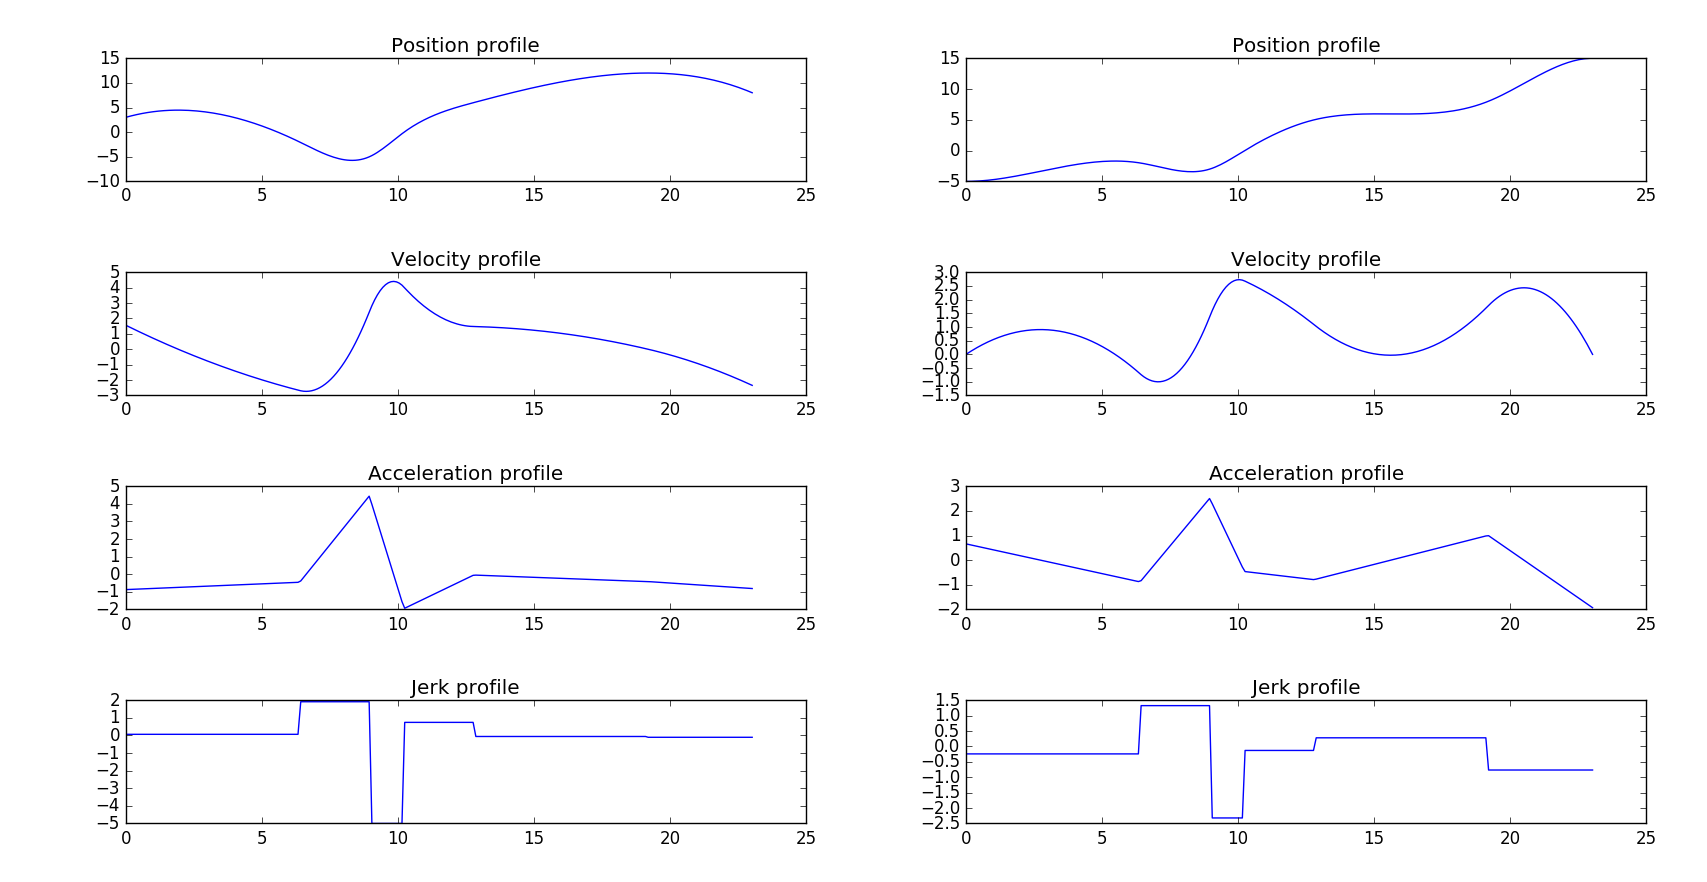
\includegraphics[scale=0.35]{TrajectoryPlanning/cubic_multipoint}
	\caption{Интерполяция и параметризация траектории от времени}
\end{figure}

Как видно из рисунка, данный метод не обеспечивает непрерывности ускорений в начале и в конце движения, что может быть неприемлемо в некторых задачах. В этом случае можно интерполировать всю траекторию или же только первый и последний участок полиномами пятой степени.


\section{Планирование траекторий между двумя точками без обхода препятствий} \label{sect5_3}

\subsection{Планирование без обхода препятствий} \label{subsect5_3_1}
	Существует огромное количество способов спланировать траекторию между двумя точками без обхода препятствий, но мы остановимся на одном из самых популярных выборов для этой задачи - double S-curve траектории, которые обеспечивают гладкость функции положения и скорости, а также непрерывность функции ускорения. Рывок в свою очередь разрывен, но ограничен максимальным значением.

	Ограничения накладываемые на траекторию: $v_{max},\ a_{max},\ j_{max}$.
	
	Кроме того выбор начальной и конечной скоростей $v_{0}$ и $v_{n}$ остается за нами, а вот начальное и конечное ускорения $a_{0}$ и $a_{n}$ равны нулю.\\
	
	Траектория имеет три фазы:
	\begin{itemize}
		\item Фаза ускорения $t \in [0,T_{a}]$
		\item Фаза максимальной скорости $t \in [T_{a}, T_{a} + T_{v}]$
		\item Фаза замедления $t \in [T_{a} + T_{v}, T]$, где $T = 2T_{a} + T_{v}$
	\end{itemize}

	Не всегда можно построить траекторию, удовлетворяющую всем наложенным ограничениям. Например, если требуемый путь мал по сравнению с разницей начальной и конечной скоростей, то может оказаться невозможным удовлетворить начальным и конечным значениям скоростей из-за ограничений на максимальные значения ускорения и рывка. В данном случае в траектории присутствует только одна фаза ускорения. Поэтому перед расчетом траектории необходимо убедиться в том, что траекторию можно построить последовательными импульсами рывка: одним - положительным и вторым - отрицательным. Для проверки положим:
	\[
	T_{j}^{*} = min \left\{ \sqrt{\frac{|v_{1} - v_{0}|}{j_{max}}},\ \frac{a_{max}}{j_{max}} \right\}
	\]
	
	Если $T_{j}^{*} = \frac{a_{max}}{j_{max}}$, ускорение достигает своего максимального значения и участок с нулевым рывком может присутствовать в траектории. Кроме того, траектория может быть построена только при выполнении следующих условий:
	
	\begin{align} \label{eq5_3_1_1}
		q_{1} - q_{0} >
		\begin{cases}
			T_{j}^{*}(v_{0} + v_{1}),				&\text{если } T_{j}^{*} < \frac{a_{max}}{j_{max}}\\
			\frac{1}{2}(v_{0} + v_{1}) \left[ T_{j}^{*} + \frac{|v_{1} - v_{0}|}{a_{max}} \right],	&\text{если } T_{j}^{*} = \frac{a_{max}}{j_{max}}
		\end{cases}
	\end{align}

	Если неравенство \ref{eq5_3_1_1} выполняется, то могут произойти два случая. Пусть $v_{lim} = max(\dot{p(t)})$, тогда:
	\begin{itemize}
		\item Случай 1: $v_{lim} = v_{max}$
		\item Случай 2: $v_{lim} < v_{max}$
	\end{itemize}
	
	Теперь определим продолжительности каждой из фаз траектории, рассмотрев оба случая. Для начала определим искомые параметры:
	\begin{align*}
	&T_{j1}		&-	& \text{ Время интервала в фазе ускорения, на котором рывок постоянен.}\\
	&T_{j1}		&-	& \text{ Время интервала в фазе замедления, на котором рывок постоянен.}\\
	&T_{a}		&-	& \text{ Время ускорения.}\\
	&T_{v}		&-	& \text{ Промежуток, на котором скорость постоянна.}\\
	&T_{d}		&-	& \text{ Время замедления.}\\
	&T			&-	& \text{ Полное время траектории}
	\end{align*}

	\textbf{Случай 1: $v_{lim} = v_{max}$}\\
	В этом случае есть возможность определить, достигается ли максимальное ускорение:
	\begin{align}
		\text{Если } (v_{max} - v_{0})j_{max} < a_{max}^{2} \rightarrow \text{ускорение не достигает } a_{max} \label{eq5_3_1_2} \\		
		\text{Если } (v_{max} - v_{1})j_{max} < a_{max}^{2} \rightarrow \text{ускорение не достигает } a_{max} \label{eq5_3_1_3}
	\end{align}

	Если неравенство \ref{eq5_3_1_2} выполняется, то временные интервалы в фазе ускорения можно вычислить следующим образом:
	\begin{align}
		T_{j1} = \sqrt{\frac{v_{max} - v_{0}}{j_{max}}},\ T_{a} = 2T_{j1}
	\end{align}
	в противном случае:
	\begin{align}
		T_{j1} = \frac{a_{max}}{j_{max}},\ T_{a} = T_{j1} + \frac{v_{max} - v_{0}}{a_{max}}
	\end{align}

	Временные интервалы фазы замедления, в случае выполнения неравенства \ref{eq5_3_1_3}, можно вычислить по следующим формулам:
	\begin{align}
		T_{j2} = \sqrt{\frac{v_{max} - v_{1}}{j_{max}}},\ T_{d} = 2T_{j2}
	\end{align}
	в противном случае:
	\begin{align}
		T_{j1} = \frac{a_{max}}{j_{max}},\ T_{d} = T_{j2} + \frac{v_{max} - v_{1}}{a_{max}}
	\end{align}

	Наконец, можно определить длину промежутка с константной скоростью:
	\begin{align}
		T_{v} = \frac{q_{1} - q_{0}}{v_{max}} - \frac{T_{a}}{2}(1 + \frac{v_{0}}{v_{max}}) - \frac{T_{d}}{2}(1 + \frac{v_{1}}{v_{max}})
	\end{align}

	Если $T_{v} < 0$, это означает, что $v_{lim}$ на самом деле меньше $v_{max}$ и необходимо рассмотреть второй случай.
	
	\textbf{Случай 2: $v_{lim} < v_{max}$}\\
	В этом случае фаза с постоянной скоростью отсутствует($T_{v} = 0$). Если максимальное(минимальное) значения достигаются, то временные интервалы ускорений и замедлений могут быть вычислены:
	\begin{align} \label{eq5_3_1_4}
	T_{j1} = T_{j2} = T_{j} = \frac{a_{max}}{j_{max}}
	\end{align}
	а полное время участков:
	\begin{align} \label{eq5_3_1_5}
		T_{a} = \frac{\frac{a^{2}_{max}}{j_{max}} - 2v_{0} +\sqrt{\Delta}}{2a_{max}}
	\end{align}
	\begin{align} \label{eq5_3_1_6}
		T_{d} = \frac{\frac{a^{2}_{max}}{j_{max}} - 2v_{1} +\sqrt{\Delta}}{2a_{max}}
	\end{align}
	где
	\begin{align} \label{eq5_3_1_7}
		\Delta = \frac{a^{4}_{max}}{j_{max}^{2}} + 2(v_{0}^{2} + v_{1}^{2}) + a_{max}\left( 4(q_{1} - q_{0}) - 2\frac{a_{max}}{j_{max}}(v_{0}+v_{1}) \right)
	\end{align}

	Если $T_{a} < 2T_{j}$ или $T_{d} < 2T_{j}$, то максимальное(минимальное) ускорения не достигаются. В этом случае вычислить траекторию, используя уравнения \ref{eq5_3_1_4}, \ref{eq5_3_1_5}, \ref{eq5_3_1_6}, \ref{eq5_3_1_7}, не представляется возможным. Но решение все же есть: можно уменьшать максимальное ускорение $a_{max}' = \gamma a_{max}$, где $0 < \gamma < 1$, до тех пор, пока траектория не построится.
	
\subsection{Синхронизация траекторий во времени} \label{subsect5_3_2}
Когда траектория строится для нескольких степеней свободы одновременно, то в случае, если конечная скорость для одной из них ненулевая, требуется синхронизация траекторий во времени. При этом заранее невозможно определить, какая из траекторий будет отработана быстрее, для этого требуется полный расчет каждой из траекторий, что может потребовать больших вычислительных ресурсов. Если предположить, что начальные скорости малы относительно требуемых перемещений, то с большой вероятностью траектория с наибольшим требуемым перемещением будет отрабатываться дольше всего. Посколько все траектории оптимальны во времени, построить ее так, чтобы она требовала меньше времени невозможно, но возможно "замедлить" траектории для оставшихся степеней свободы, используя тот же самый метод с уменьшением максимального ускорения на каждой итерации $a_{max}' = \gamma a_{max}$.

\subsection{Результаты} \label{subsect5_3_3}
Построим траекторию в трех степенях свободы:
\begin{align*}
	q_{0} = \{-2, 0, 10\},\ q_{1} = \{20, 85, -10\}\\
	v_{0} = \{0, 5, 0\},\ v_{1} = \{2, 4, 0\}\\
	v_{max} = 30,\ a_{max} = 30,\ j_{max} = 100
\end{align*} 

\begin{figure}[ht]
	\centering
	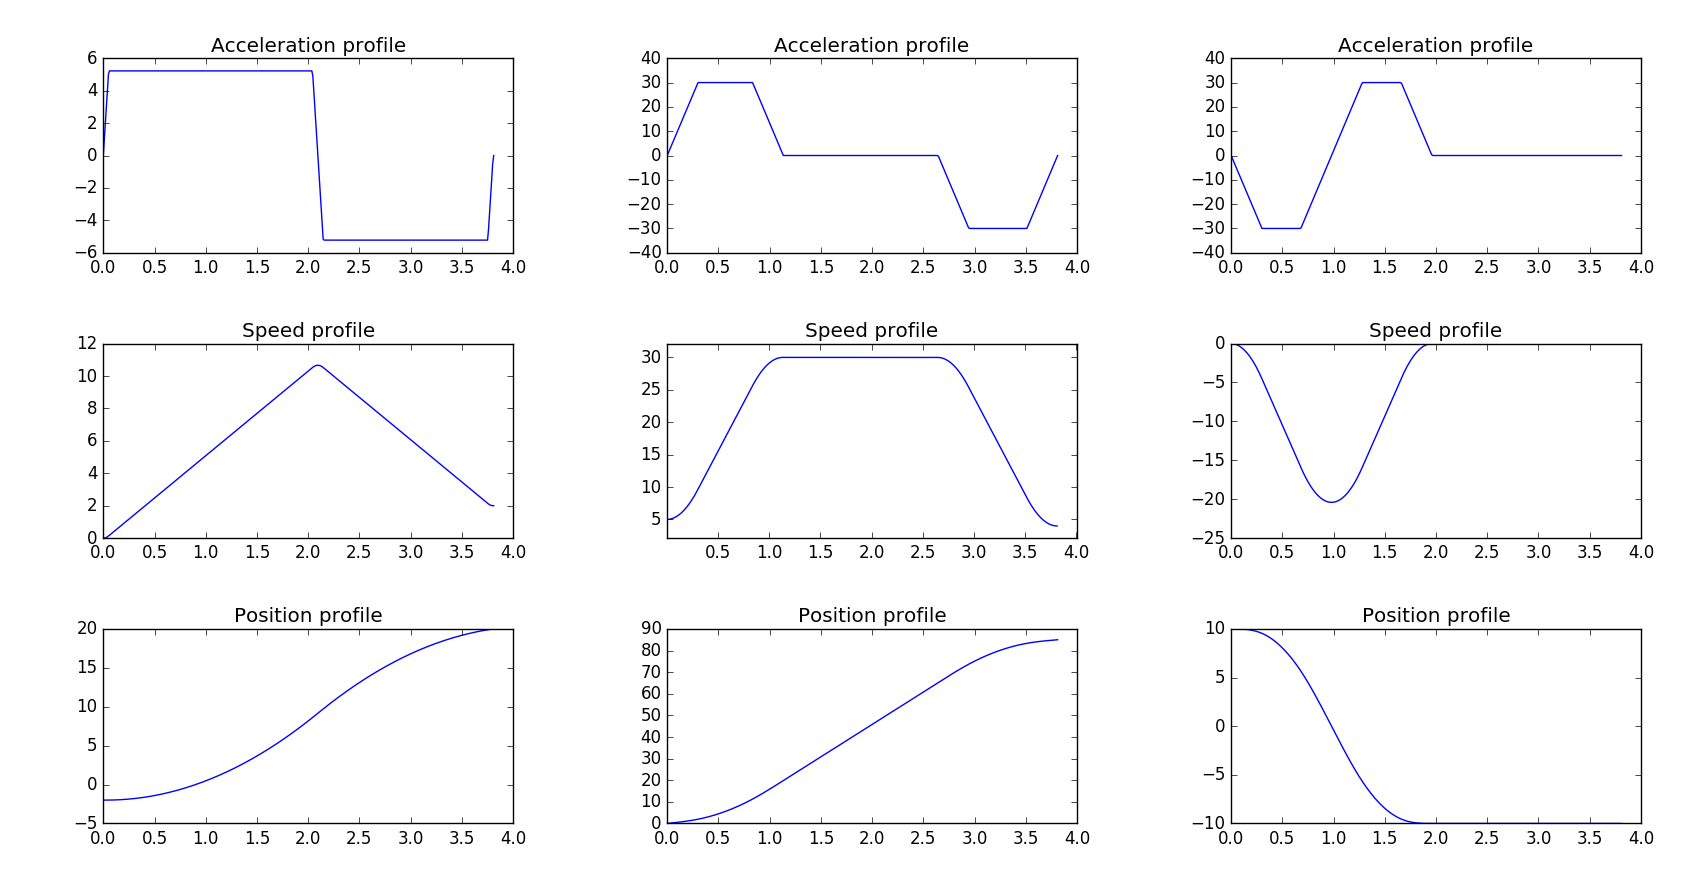
\includegraphics[scale=0.35]{TrajectoryPlanning/pyscurve_ex0}
	\caption{Double s-curve траектория для точки имеющей три степени свободы}
	\label{fig:pyscurve_ex0}
\end{figure}

Результат представлен на рисунке \ref{fig:pyscurve_ex0}.
Как видно из графиков, первые две траектории синхронизированы во времени, поскольку имеют ненулевые конечные скорости. В то же время для третьей - построена оптимальная во времени траектория, поскольку она имеет нулевую конечную скорость. Кроме того из первых двух наиболее продолжительной является вторая траектория, поэтому для нее расчитана оптимальная во времени траектория, в то время, как первая - "замедлена" до требуемого времени исполнения.